\documentclass[12pt]{article}

\usepackage[utf8]{inputenc}%encodage des caractères
\usepackage[T1]{fontenc}%encodage de la police
\usepackage[french]{babel}%langue française
\usepackage{hyperref}
\usepackage{amsmath}
\usepackage{graphicx}
\usepackage[linesnumbered,ruled,french,onelanguage]{algorithm2e}
\usepackage{color}


\title{\underline{
		Rapport du Projet Ricochet Robot}
	\underline{
		\\Travail Personnel Approfondi}}
\author{Bamba Alassane
	\\Camara Mohamed
	\\Komara Mohamed Ba
	\\Salami Sodiki Olawale}
\date{\today}


\begin{figure}[b]
	L2 Informatique 
	\\Année 2019-2020
\end{figure}

\begin{document}
\maketitle
\newpage
		\tableofcontents
		\newpage
		
		\section{Introduction}


		L’unité́ d’enseignement de TPA (Travail Personnel Approfondi) a pour objectif de nous faire comprendre le concept de la programmation orientée objet, nous initiés aux algorithmes d’intelligence artificielle et parfaire notre maitrise de java. 
		\\Pour cela des groupes de 4 d’étudiants ont été formés et plusieurs projets ont été proposés, Éditeur de livres dont vous êtes le héros, Générateur de flores vidéos-ludique, Interpréteur de programmes chimiques, etc.
		Notre groupe a choisi le projet Ricochet Robot 
		
		
		
			\subsection{Ricochet Robot}
			
			Ricochet Robots (Rasende Roboter pour la première édition en allemand) est un jeu de société créé par Alex Randolph et illustré par Franz Vohwinkel, édité en 1999 par Hans im Glück / Tilsit.
			\\Le principe du jeu de société Ricochet Robots est de trouver en moins d'une minute la séquence de mouvement qui permettra à un robot donné (parmi quatre) d'atteindre un objectif désigné sur une case du plateau de jeu. Cependant, les robots ne peuvent que se déplacer en ligne droite jusqu'à rencontrer un obstacle.
		
			\subsection{Objectif du projet}
			
			Le but de ce projet est de développer un programme permettant de trouver une solution optimale pour toute situation du jeu. Dans un premier temps, il s'agira de développer le moteur du jeu (cf. règles) puis d'implanter un algorithme de résolution naïf, appelé A*. Cependant, le problème est trop complexe pour être résolu dans de bonnes conditions. Dans un second temps, il s'agira alors de proposer des méthodes d'optimisation de l'algorithme, par exemple en utilisant des tables de transposition. Enfin, s'il reste du temps, il pourra être intéressant de réaliser une interface graphique permettant à un utilisateur de sélectionner un objectif. 
			
		\section{Organisation de projet }
			\subsection{Répartition des taches }
			
			
			Dans un premier temps, nous avons décidé de travailler ensemble pour essayer de bien comprendre le projet, identifier les objectifs et élaborer un plan de travail.
			A la suite de cette première phase de travail on a identifié et classifié dans l’ordre de priorité les différents objectifs :
			\\Dans un premier temps, nous avions cherché à modéliser les digrammes de classe sur lesquels se basera le jeu, et développer le moteur du jeu basé sur les règles du jeu. Puis une interface graphique permettant à l’utilisateur de jouer.   
			\\Dans un second temps nous avons implanter un algorithme de résolution naïf, appelé A*.
			
			Pour atteindre nos objectifs à temps et permettre à chacun d’entre nous de bien comprendre le projet, nous nous sommes séparés en binômes. Mohamed Ba Komara et Alassane Bamba se sont concentrés sur le monteur de jeu et l’algorithme A étoile, tandis que Mohamed Camara et Salami Sodiki Olawalé ont actés à la réalisation de l’interface graphique. . Pour faciliter ce travail de groupe nous avons eu à se trouver souvent pour travailler avant le début des confinements et nous avons souvent utilisés une application appelée Team Viewer qui facilité le travail de groupe, mais depuis début du confinement nous travaillons essentiellement à travers cette application. 
			
			
			\subsection{Architecture du programme }
			
				
			Pour ce projet nous avons opté pour une architecture MVC (Modèle Vue Contrôleur). Nous avons donc décomposé le projet en 5 packages :
			\\\textbf{PackageRR :} Il contient toutes les classes utilisées comme model de jeu à savoir la classe Case, Cible, Direction, Plateau, Robot etc.
			\\\textbf{PackageRR.ihm : } Dans ce package se trouve toutes les classes de la Vue.
			Images : Qui contient toutes les images utiliser dans ce projet 
			\\\textbf{PackageAEtoile : } Ce package contient les classes d’implémentation de l’algorithme de résolution naïf A*
			\\\textbf{PackageRR.execution:}  Ce package contient les classes d'execution du jeu.
			\\Avec cette architecture nous avons obtenus les diagrammes de classes suivants :
			

			%Le premier digramme	
			\begin{figure}[htpb]
					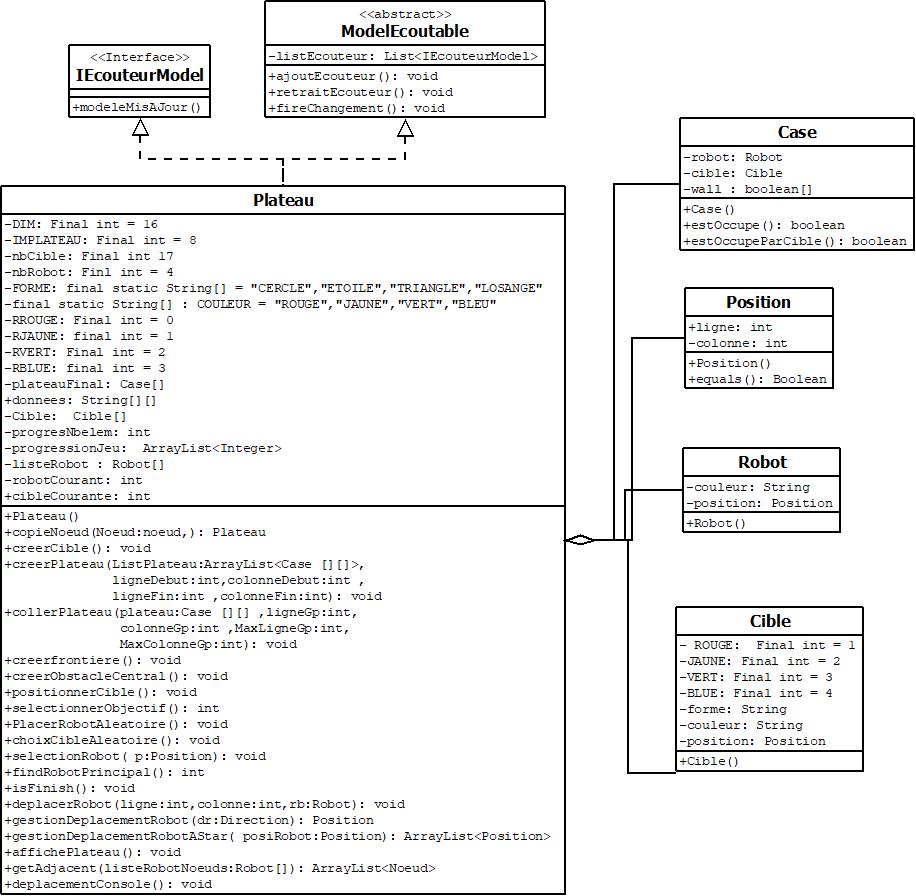
\includegraphics[scale=0.7]{./images/rr.jpg}
						\caption{Diagramme des classe du PackageRR \label{figure1} }
			\end{figure}
			
			\newpage
			%Le deuxieme digramme
			\begin{figure}[htpb]
				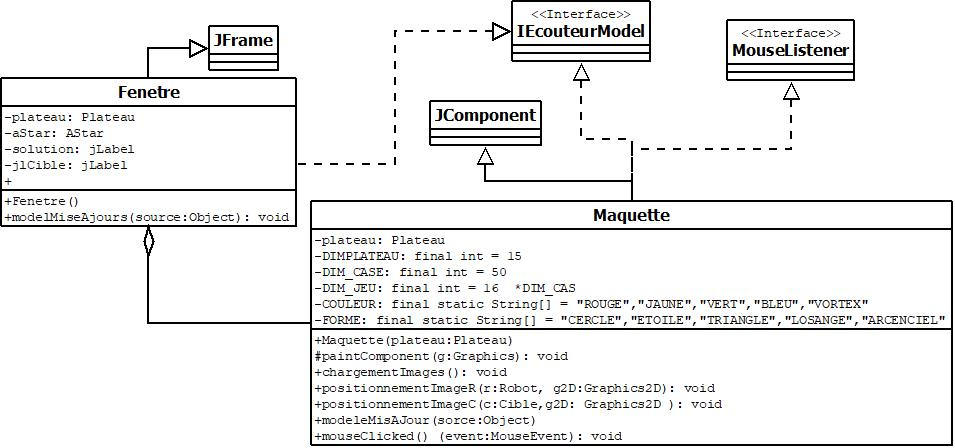
\includegraphics[scale=0.6]{./images/ihm.jpg}
				\caption{Diagramme des classe du PackageRR.Ihm}
			\end{figure}
		
		\newpage
		%Le troisieme digramme
		\begin{figure}[htpb]
			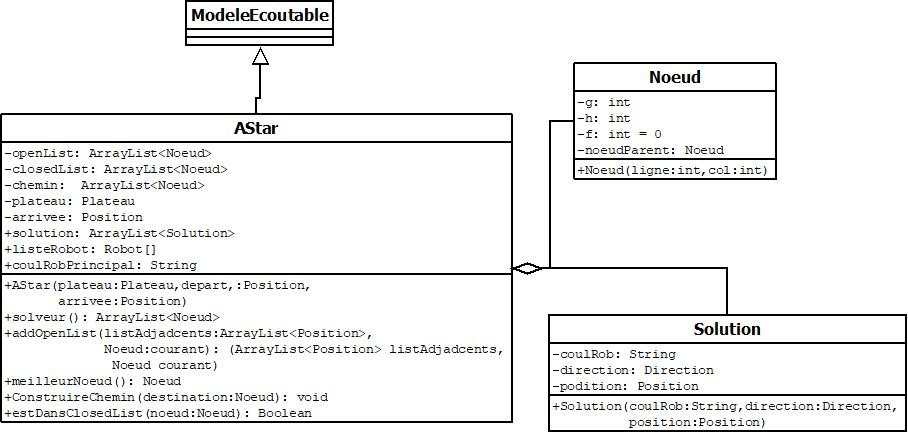
\includegraphics[scale=0.7]{./images/a.jpg}
			\caption{Diagramme des classe du PackageAEtoile}
		\end{figure}
			
			\newpage
		%Le quatrieme digramme
		\begin{figure}[htpb]
			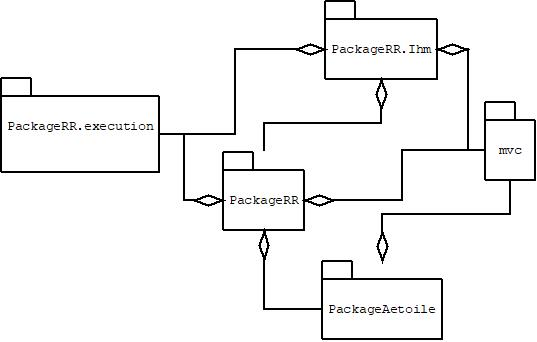
\includegraphics[scale=0.9]{./images/p.jpg}
			\caption{Diagramme des Packages}
		\end{figure}
		\newpage
			
		\section{Éléments techniques}
			\subsection{Moteur du jeu basé sur les règles}
			
			Le moteur du jeu est une partie très importante de ce projet, il représente la base du jeu. Il contient les classes comme la classe Case qui représente chaque case du jeu et qui contient les informations sur les cases (présence d’un mur gauche, droit, haut, bas, d’un robot ou encore d’une cible potentielle). La classe Robot représente les robots du jeu (Rouge, Blue, Jauge et Vert) qui se déplacent sur le plateau d’une case à une autre. 
			\\Construction du plateau :
			\\La classe Plateau est celle qui utilise toutes ces classes préalablement définies, elle contient également des méthodes comme celle qui permettent de construire le plateau du jeu.
			\\Pour la réalisation du plateau nous avions effectué un certain nombre de codages.
			\\Dans un premier temps nous avions créé un tableau a deux dimensions de 16 sur 16 de chaine de caractères dans lequel est représenté la disposition initiale des murs et des cibles. 
			\\En effet cette disposition se fait de manière suivante :
			\\Le mot Null dans le tableau représente les cases vides
			\\Pour les cases non vides nous avons procédé au codage suivant : 0 0 0 0 17
			\\D’où 
:
			\\La première valeur représente le mur du haut, (0 pour l’absence du mur ou 1 pour la présence du mur).
			\\La deuxième valeur représente le mur droit 
			\\La troisième valeur représente le mur du bas
			\\La quatrième valeur représente le mur gauche
			\\La dernière valeur présente l’une des dix-sept cibles possibles.
			\\Dans un second temps nous créons les quatre petits plateaux à partir de ce grand tableau, puis nous effectuons des permutations puis nous collons ces petits plateaux pour former à la fin un grand plateau de 16 sur 16. A la suite de cela nous dessinons les frontières du jeu (les murs qui forment les bordes du jeu) puis l’obstacle central (les murs du sont au centre du plateau). En ce qui concerne les places des robots, elles sont également choisies de façon aléatoire mais contrôler de tel sorte qu’un robot ne se place jamais à la place d’une cible.
			\\La méthode selectionnerObjectif () choisit aléatoirement une cible parmi les 17 cibles possibles de façon à ne pas choisir deux fois une même cible.
			
			
			
			\subsection{L’interface graphique}
			
			Pour réaliser l’interface graphique, nous avons utiliser un JFrame pour avoir une fenêtre dans laquelle on a placé à l’Est un JPanel qui contient  quatre JButton permettant de faire les déplacements des robots dans les quatre directions possibles. 
			En suite au centre nous avions placé un JComponent Maquette contenant la grille (le plateau).
			Maquette est une classe qui hérite de JComponent à partir de laquelle nous importons les images du package Images représentant certains objets du jeu comme les robots, les cases, et les cibles grâce à la méthode chargementImages(). Chaque image est dessinée en fonction de la case ou du robot correspondant et à la place de chaque mur du model, un rectangle est dessiné à ce niveau pour les obstacles.
			
			
		\subsection{Algorithme de résolution naïf A étoile (A*)}
		
		L’algorithme A* est un algorithme de recherche de chemin dans un graphe entre un nœud initial et un nœud final. Il utilise une évaluation heuristique sur chaque nœud pour estimer le meilleur chemin y passant, et visite ensuite les nœuds par ordre de cette évaluation heuristique.
		\\Dans notre cas un nœud est représenté par une liste contenant la position des 4 robots, de son nœud parent et de la valeur de sa fonction d’évaluation f.
		Cette fonction est calculée comme suit :f(n)=g(n)+h(n)
		— g(n) : représentant le coût du chemin entre le nœud de départ et le nœud n
		— h(n) : représentant le coût estimé entre le nœud n et le nœud d’arrivée ;c’est l’heuristique.
		G(n) est facile à être déterminé par contre h(n) est un petit peu plus compliqué et en plus la performance d’un algorithme A* dépend beaucoup de l’heuristique.
		Dans notre cas nous avons eu a implémenté 2 heuristiques :
		\\-  La distance à vol d’oiseau
		\\-  La distance de Manhattan
		Après plusieurs tests nous avons finalement fini par pencher pour celle de Manhattan qui mettait moins de temps que celle à vol d’oiseau.
		Fonctionnement : Le fonctionnement de l’algorithme est le suivant : Nous devons tout d’abord disposer de 2 listes : OpenList et closedList.
		Openlist : contient les nœuds qui n’ont pas encore été explorés
		ClosedList : contient les nœuds déjà explorés.
		Au début de l’algorithme, on considère le nœud initial comme étant la représentation du plateau de jeu à résoudre.
		\\-Ensuite On récupère tous les adjacents ce nœud. (16 adjacents avec la configuration actuelle)
		\		\-On ajoute tous ces adjacents dans l’openList du coup le nœud initial est ajouté à la closedList
		\\-Ensuite On récupère le meilleur nœud dans l’openList; c’est-à-dire celui qui a la plus petite valeur de f(n) et on  le supprime de cette liste pour l’ajouter dans la closedList.Donc tous les adjacents de ce nœud seront  à leur tour ainsi étudiés :
		           \\ 1-  vérifier l’existence du nœud dans la closedList
		           \\2-  S’il n’y existe pas on l’ajoute dans l’openList
		          \\ 3-  Dans le cas contraire ,il y  existe donc on passe au nœud suivant ; cela voudrait dire qu’il a déjà été étudié.
		En gros on répète ces itérations successives jusqu’à atteindre un nœud où la position du robot principal sera identique à celle de la cible choisie ou jusqu’à vider l’openList.
		Une fois la solution obtenue on utilise la méthode construireChemin(courant) qui va parcourir la closedList de façon à reconstruire le chemin qui aboutit à la solution.  
		
		\newpage
		\begin{algorithm}
			
			\caption{A Etoile}
			\KwIn{
				\text{\bf Initialisations }:
				\\Sommet Source (S)
				\\Sommet Destination (D)
				\\Liste ouverte à explorer (E) : sommet source S
				\\Liste fermée deja visités (V): vide
			}
			
			\While{$E != \emptyset$ \vee  $D n'est pas dans  $ E}{
				$X \gets meilleur Noeud_$\;
				\\Ajouter X  dans la liste
				\\Ajouter les successeurs de X (Non deja visité) a E
				en evaluant leur cout F et en identifiant leur predecesseur
				\\
				\If {(un successeurs est deja present dans $E )\vee  (Nouveau Cout < L'ancien)}{
					
					$Changer son cout F $\;
					$Changer son predecesseur $\;}
			}
		\end{algorithm}
		
		
		\subsection{Manuel d'utilisation }  
			Le jeu ricochet robot a pour objectif principal de faire parvenir les robots à leur cible correspondante.
			Une fois l'application lancée, une cible est choisie aléatoirement parmi les 17 possibles, puis nous devons déplacer les robots jusqu'a ce que le robot correspondant atteingne la cible  choisie.
			
		\newpage
		%--Afficher image Fenetre principale du jeu
			\begin{figure}[htpb]
			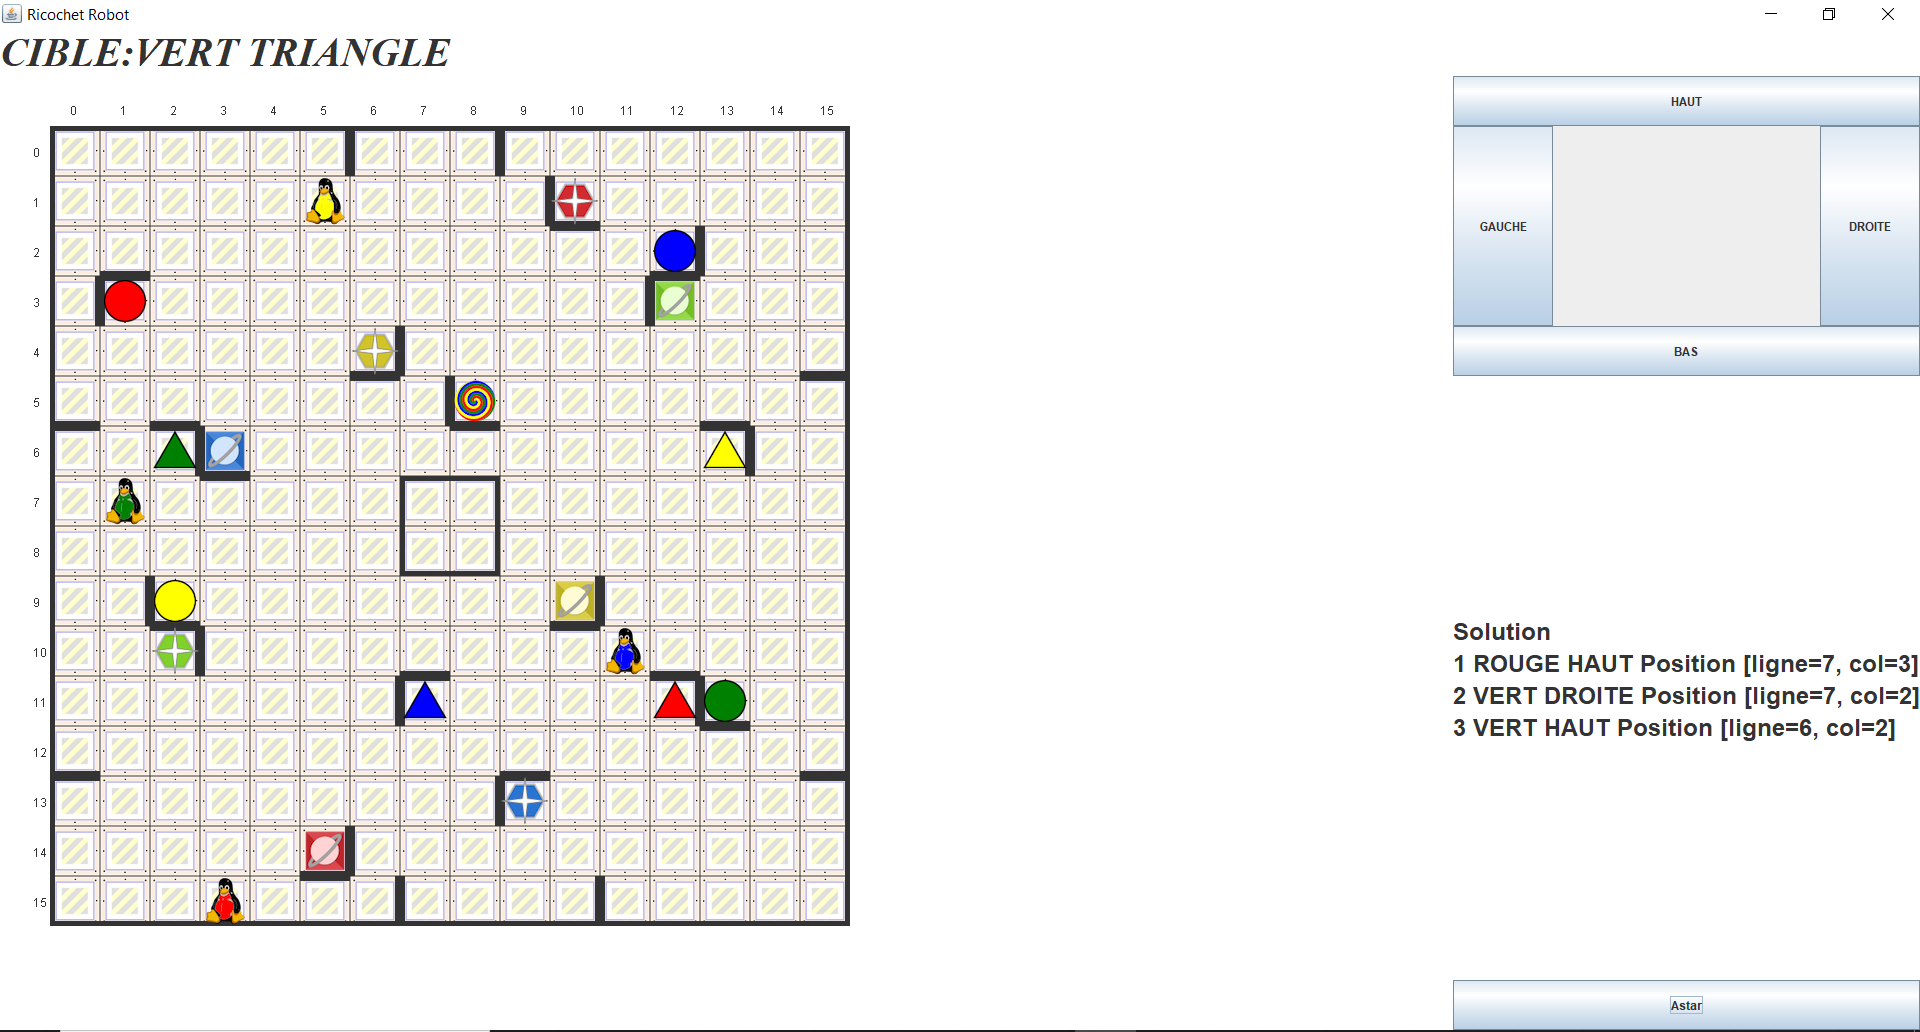
\includegraphics[scale=0.4]{./images/g.png}
			\caption{Fenetre principale du jeu}
			\end{figure}
			
	\newpage
			%--Afficher  du plateau dans la console
			\begin{figure}[htpb]
			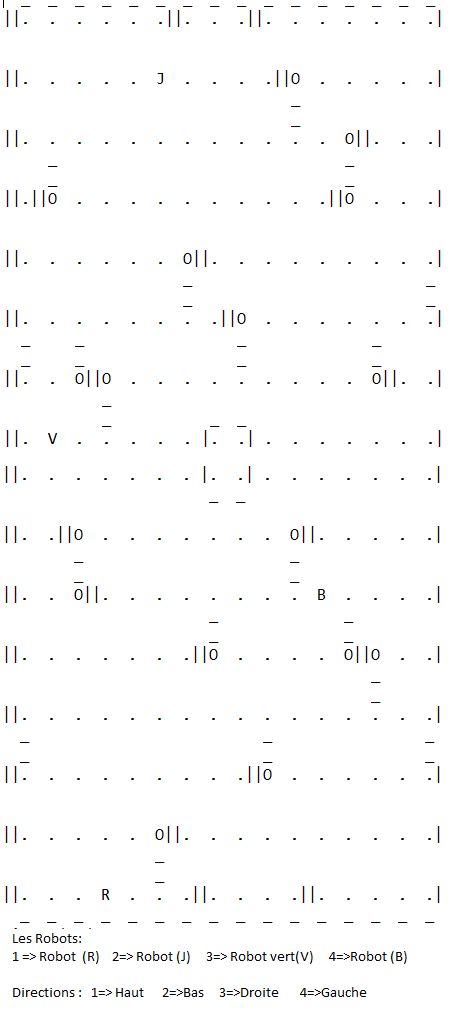
\includegraphics[scale=0.5]{./images/jeuConsole.png}
			\caption{Affichage dans la console}
			\end{figure}
			

		\newpage
			Pour déplacer un robot, il faut tout d'abord cliquer sur le robot avec la souris puis cliquer sur l'une des quatre direction possibles sur la fenêtre (Haut, Gauche, Droit, Bas).
		
		%--Afficher les touches de controles
		\begin{figure}[htp]
			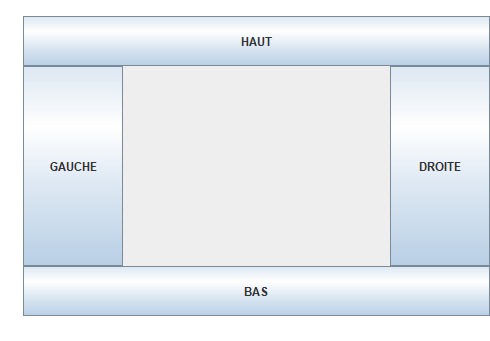
\includegraphics[scale=0.6]{./images/btnControl.png}
			\caption{Les touches de déplacements}
		\end{figure}	
			
			Si aucun des joueurs n'arrive à trouver une solution pour envoyer le robot correspondant à la cible aléatoirement choisi, on peut ainsi cliquer sur le bouton Astar.
			
			\begin{figure}[htpb]
				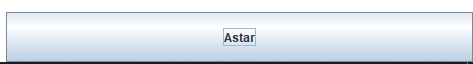
\includegraphics[scale=0.6]{./images/btnAstar.png}
				\caption{Bouton AStar}
			\end{figure}
			
				Le bouton AStar proposera une solution c'est à dire proposera les bonnes positions auxquelles il faut déplacer les robots pour résoudre le problème.
		
		
			\\newpage
			\begin{figure}[htpb]
				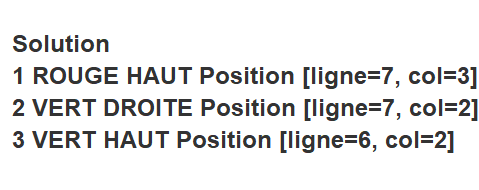
\includegraphics[scale=0.6]{./images/solutionAEtoil.png}
				\caption{Bouton AStar}
			\end{figure}
			
			Les joueurs devront déplacer les robots en respectant les positions proposées par AStar. 
			\\Une fois que le robot atteint sa destination, une autre cible sera encore aléatoirement choisi jusqu'à la fin des 17 cibles possibles et le même processus reprend jusqu'à l'épuisement des cibles qui mettra fin à la partie.
			
		
		\section{Conclusion }
		La réalisation de ce projet a été une occasion pour nous membre de ce groupe d’apprendre encore plus le langage de programmation Java.
		Pendant ce projet, nous avons pu appliquer ce que nous avions appris dans les CM, les TP de ce semestre et ceux du semestre passé à savoir : la programmation orientée objet, la conception d’applications, les algorithmes récursifs et l’implémentation des algorithmes d’intelligence artificielle. 
		\\D'un point de vue humain, nous avons appris à mieux travailler en équipe, à communiquer, à bien organiser un travail d’équipe et le plus important à combler nos lacunes.  
		Nous avons également appris à travailler à distance en utilisant les outils de travail de groupe comme TEAM VIEWER et SVN.
		
			\subsection{Objectifs remplis }
			
			Dans ce projet, nous avions pour objectifs de réaliser le jeu Ricochet-Robots en implémentant toutes les règles du jeu dans une application JAVA et d’y implémenter l’algorithme de résolution naïf A*. Nous avons donc pu coder le moteur du jeu respectant toutes les règles du jeu, nous avons aussi réussi par faire une interface graphique afin que le jeu soit jouable pour un ou plusieurs joueurs, en jouant à l’aide des quatre buttons de déplacement, ainsi que l’affichage d'une solution possible en déplaçant les quatre robots avec l’algorithme de résolution naïf A*. 
			
			\subsection{Améliorations possibles   }
			
			Nous pouvons ameliorer cette application à plusieurs niveaux; tout d'abord  trouver une meilleure heuristique pour l'algorithme de resolution naïf A*.
			\\Puis ajouter un compteur du nombre de coups et du nombre de victoires sur l’interface graphique et  un chronomètre. Nous pourrions également y ajouter un menu principal et porter le jeu sous mobile. 
			\\L’interface graphique peut être améliorer en affichant sur le plateau le parcours de la meilleure solution.
			
			
			
			
\end{document}